\section{Problem 4}

\subsection{a}

\begin{figure}[H]
 \centering
 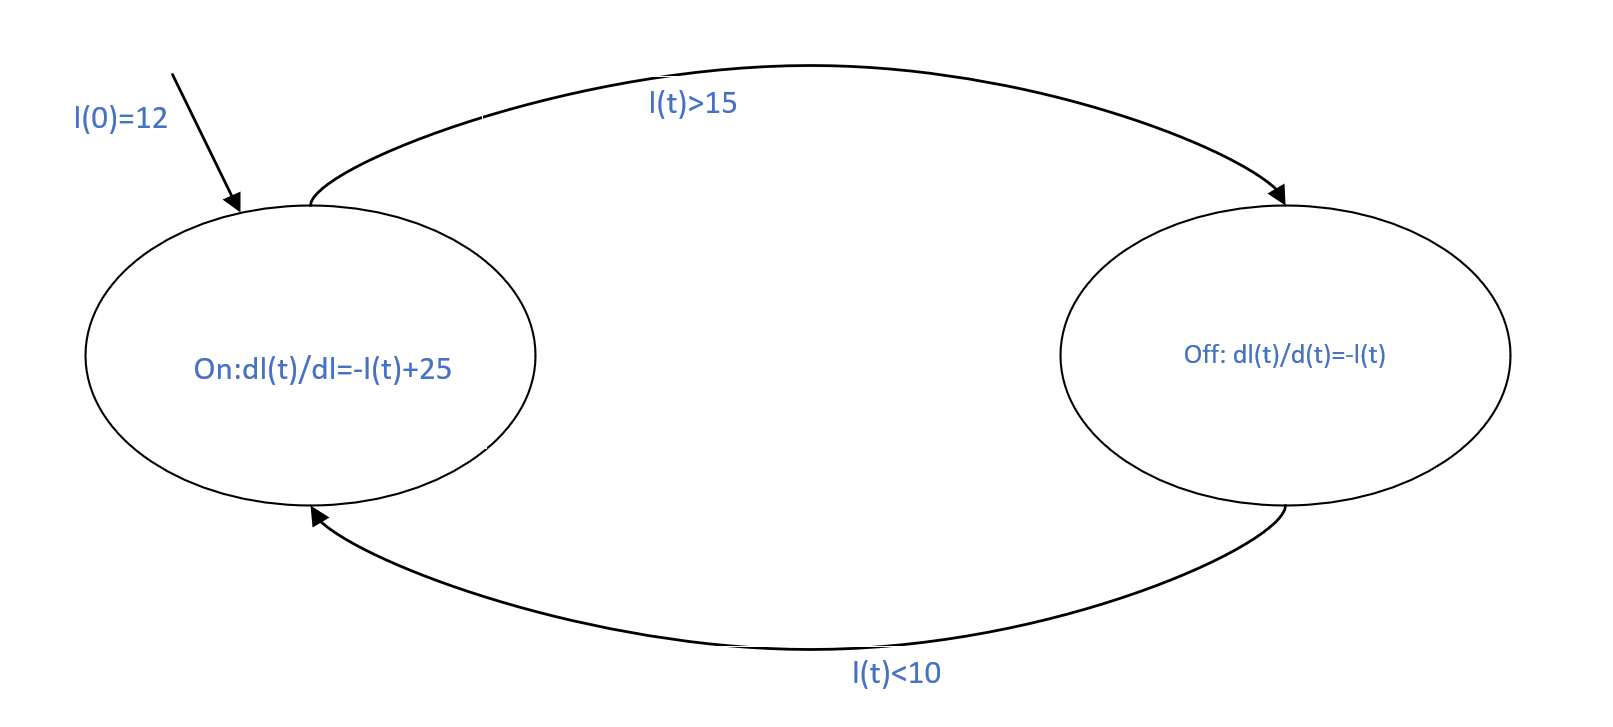
\includegraphics[width=0.9\textwidth]{images/automataa.png}
 \caption{Automata}
 \label{a}
\end{figure}

\subsection{b}

I used Simulink to do this modeling:
\begin{figure}[H]
 \centering
 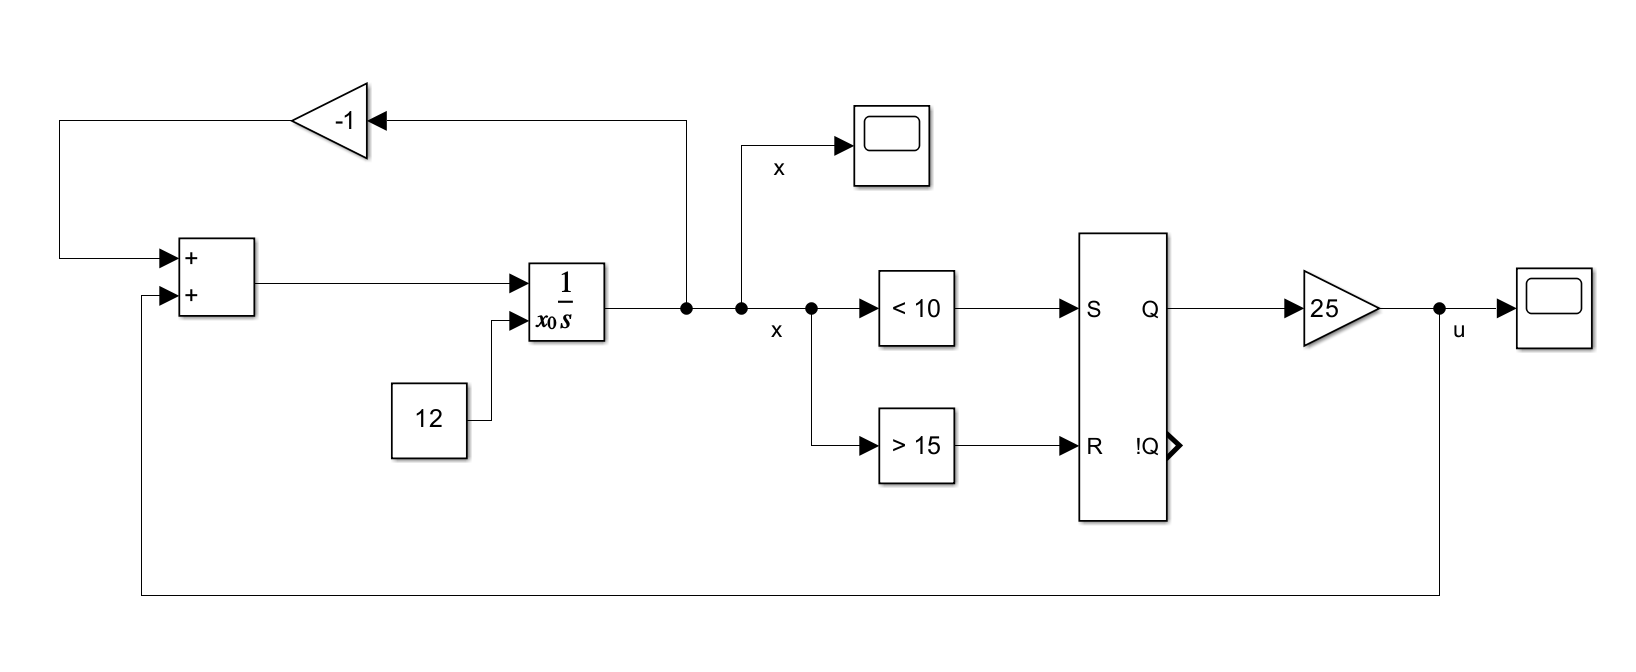
\includegraphics[width=0.9\textwidth]{images/model.png}
 \caption{Model in Simulink}
 \label{model}
\end{figure}

Here in figure \ref{compare-zero-crossing} shows the difference between with and without zero-crossing detection enabled with variable step solver.

\begin{figure}[h]
    \centering
    \begin{subfigure}[b]{0.9\textwidth}
        \centering
        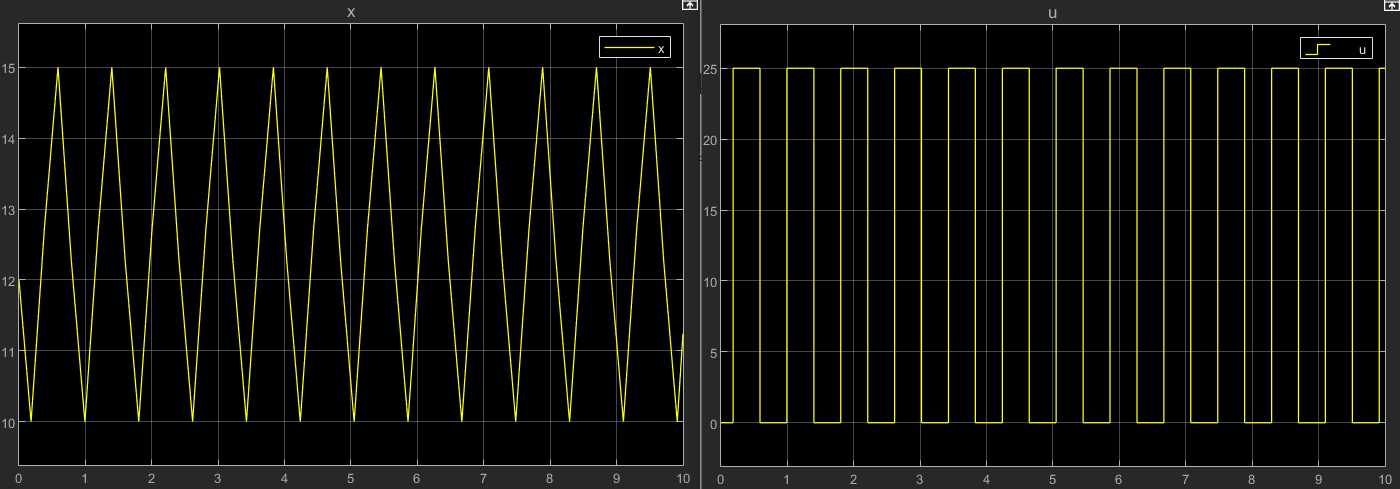
\includegraphics[width=\textwidth]{images/withzerocrossing.png}
        \caption{With Zero Crossing}
        \label{with}
    \end{subfigure}
    \hfill
    \begin{subfigure}[b]{0.9\textwidth}
        \centering
        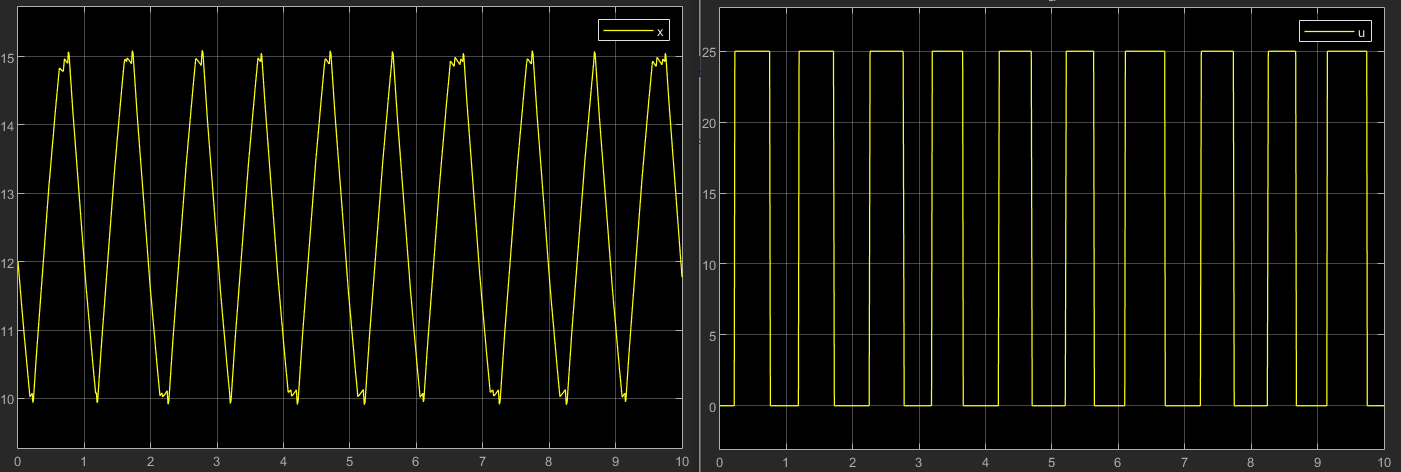
\includegraphics[width=\textwidth]{images/withoutzerocrossing.png}
        \caption{Without Zero Crossing}
        \label{without}
    \end{subfigure}
    \caption{Comparison of Zero Crossing on/off for variable step}
    \label{compare-zero-crossing}
\end{figure}

As you can see, there is a 'shake' on the peak, but it is not easy to analyze and it can not match the lecture.

Now to change the solver to Fixstep:

\begin{figure}[h]
    \centering
    \begin{minipage}{.5\textwidth}
      \centering
      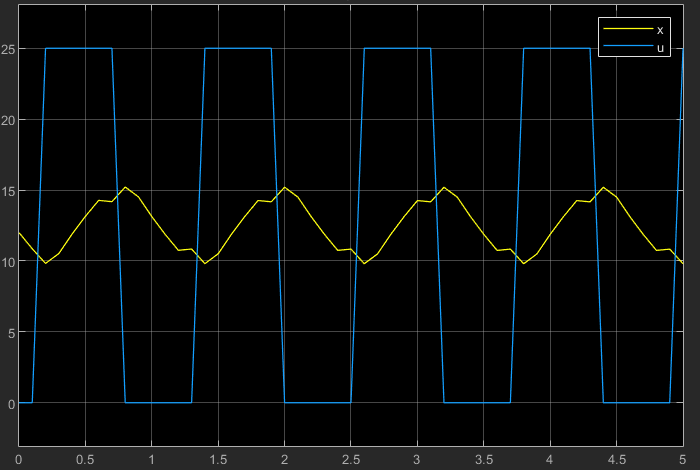
\includegraphics[width=0.8\linewidth]{images/disableall.png}
      \caption{Off}
      \label{disableall}
    \end{minipage}%
    \begin{minipage}{.5\textwidth}
      \centering
      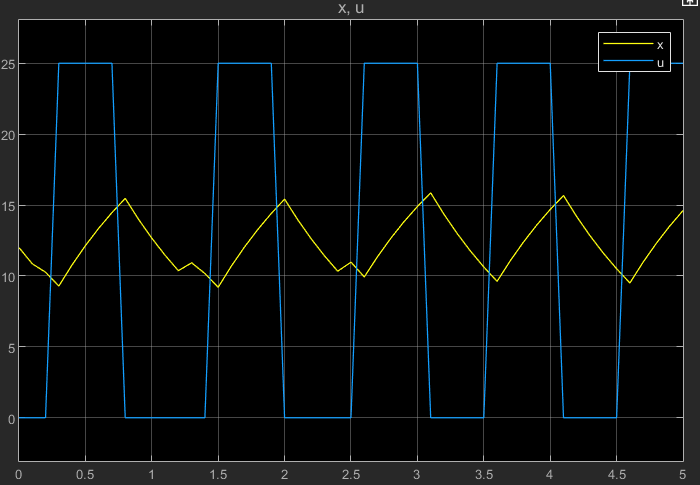
\includegraphics[width=0.8\linewidth]{images/enabledall.png}
      \caption{On}
      \label{enabledall}
    \end{minipage}
    \caption{Comparison of Off and On in Fixstep}
    \label{offandon}
    \end{figure}

    We can see it is obvious with the zero-crossing option enabled the state curve becomes smooth at the edge of the control signal u.

\subsection{c}

Zeno behavior occurs when the system appears to repeatedly approach a limit or event horizon without actually reaching it, but in our system, there is a gap between two event horizons so the Zeno behavior cannot approach.